\section{Определение стохастичности в модели с ротационной симметрией}

\subsection{Сечения Пуанкаре}
~\par
%Для обнаружения и исследования хаотических движений были построены сечения Пуанкаре \cite{BinneyTremaine}.
%Определение хаотических движений ??см.Динамика Солнечной системы и Шевченко
Для выявления признаков хаотических движений, наличие которых можно было бы предполагать в модели с центральным пиком плотности, используются: показатели Ляпунова (чувствительность к изменению начальных условий); фрактальные свойства движения в фазовом пространстве, которые характеризуются сечениями Пуанкаре и фрактальными размерностями~\cite{Mun}.

Сечения (или отображения) Пуанкаре  получаются путем фиксации некоторой плоскости в фазовом пространстве, например $[R(t),\dot{R}(t)]$, и определения точек, в которых траектория пересекает плоскость симметрии $z=0$ в заданном направлении, например $\dot{R}(t)>0$. На рисунке~(Рис.~\ref{poincare}) изображены сечения, соответствующие орбитам на рисунках~\ref{orbits:1},~\ref{orbits:2}. Если сечения состоят из замкнутой орбиты, то соответсвующие движения регулярные~\cite{Mun}.

{
\begin{figure}[H]
\centering
\begin{minipage}[t]{0.8\textwidth}
\centering
\includegraphics[width=\linewidth]{D:/diploma/tex/3/res/dualPoinc.png}
\end{minipage}
\caption{Сечения Пуанкаре}\label{poincare}
\end{figure}
}
%Для построенных траекторий пробных звезд в модели~(\ref{eq:xi},\ref{xi_Rz}) были рассмотрены движения на фазовой плоскости $[R(t),\dot{R}(t)]$, %точки на плоскости отмечены в моменты $t$ прохождения плоскости симметрии $z=0$.%\cite{BinneyTremaine}

\subsection{Фрактальная размерность}


\subsubsection{Определение фрактальной меры}
~\par
Фрактальная размерность есть количественная мера фрактальной природы аттрактора. Размерность точечного множества можно определить многими способами. Опишем весьма наглядное, или геометрическое определение размерности, называемое емкостью.
Пусть $N_0$ --- некоторое распределение точек, тогда определение фрактальной размерности выглядит так:
\begin{equation}\label{FRAC_RAZM_DEFINITION}
	d_c = \lim_{l \to  0} \frac{   \ln{N(l)}   }{   \ln{(1/l)}   }
\end{equation}
где $N(l)$ --- число кубов со стороной $l$, покрывающих заданное множество. $N(l) < N_0$.
Неявно в этом определении содержится требование, согласно которому число точек в множестве должно быть большим, или $N_0 \to \infty$.\\
Точечное множество называется фрактальным, если оно имеет нецелую размерность. 
Существуют два возражения против использования емкости в качестве меры фрактальной размерности. Во-первых, емкостная размерность --- геометрическая мера, т.е. она не учитывает частоту, с которой траектория посещает элемент покрытия. Во-вторых, подсчет гиперкубов, образующих покрытие множества в фазовом пространстве, требует очень больших затрат вычислительного времени. Однако, емкостная мера остается адекватной и справедливой.~\cite{Mun}

\subsubsection{Box-counting алгоритм}
~\par
Изложим алгоритм, используя который были вычислены фрактальные размерности.\\
Пусть задано компактное множество $A \in \mathbb{R}$ объединением шаров и просуммируем их объемы (или меры в общем случае). Пусть $N(l)$ --- минимальное число шаров радиуса $l$, необходимых для покрытия компактного множества $A$. Их суммарный объем $V$ пропорционален $N(l)\cdot l^D$. При $l \to 0$, $N(l) \to \frac{\text{const}}{l^D}$. Тут логарифмируем и получаем $\ln N(l) \to \ln(\text{const}) - D\ln l$. Отсюда находим: 
$$
\frac{\ln(\text{const}) - \ln N(l)}{\ln l} \to D.
$$
При $l \to 0$ значение $\ln(\text{const})$ пренебрежимо мало по сравнению $\ln N(l)$. Таким образом приходим к определению размерности Минковского:
\begin{equation}\label{Dimension}
d_M(A) =  \lim_{l \to 0} \frac{\ln N(l)}{-\ln l}.
\end{equation}
Пусть в уравнении~\ref{Dimension} $D_M = d_M$ --- приближенное значение размерности Минковского. Запишем определение этой размерности, убрав предел, его мы будем имитировать в итерациях, в которых будет изменяться размер ячеек. Если зафиксировать размеры ячеек $l$ и рассматривать $D_M$ как неизвестное, то легко заметить, что приведенное выражение является формулой линии. Мы можем запустить цикл по различным размерам ячеек $l$ и записывать результат $D_M$. Если нанести эти результаты на график и построить линию регрессии для полученного множества данных, это значение и будет являться аппроксимацией фрактальной размерности Минковского.\\

Стоит отметить, что если верхний предел не существует, все еще можно взять супремум и инфинум, которые соотвественно определяют \textbf{верхнюю box-размерность (upper box dimension)} и \textbf{нижнюю box-размерность (lower box dimension)}. Верхняя размерность иногда называют размерностью энтропии (entropy dimension),  размерностью Колмогорова (Kolmogorov dimension), объем Колмогорова (Kolmogorov capacity), предельный объем (limit capacity) или верхняя размерность Минковского (upper Minkowski dimension). В то же время нижняя размерность так же называется нижняя размерность Минковского (lower Minkowski dimension~\cite{MINKOWSKI}).\\
\subsubsection{Связь фрактальной размерности и показателей Ляпунова}
~\par
Соотношение между фрактальной размерностью и показателями Ляпунова была установлена Капланом и Йорке~\cite{KAPLAN_AND_YORKE}. Показатели Ляпунова характеризуют для траекторий на аттракторе скорость их разбегания друг от друга, а для траекторий вне аттрактора --- скорость их приближения к аттрактору. Каплан и Йорке~\cite{KAPLAN_AND_YORKE} предложили способ вычисления размерности аттрактора по показателям Ляпунова. Для двумерного отображения такая размерность определяется по формуле:
$$
	d_L = 1 + \frac{   \log{L_1}   }{   \log{(1/L_2)}   } = 1 - \frac{\lambda_1}{\lambda_2}.
$$

Для отображений более высокой размерности в $N$-мерном фазовом пространстве связь между показателями Ляпунова и размерностью Ляпунова более сложная. Прежде всего необходимо упорядочить показатели Ляпунова, т.е. расположить их в убывающую последовательность $L_1 > L_2 > ... > L_k > L_N$, а затем найти $L_k$ такое, что $L_1L_2...L_k \ge 1$. Тогда ляпуновской размерностью по определению называется величина:
$$
	d_L = k + \frac{   \log{L_1L_2...L_k}   }{   \log{(1/L_{k+1})}   }.
$$
Так же, Каплан и Йорке высказали предположение о том, что $d_L$ является нижней границей для фрактальной размерности $d_M$, т.е. выполняется неравенство $d_L \le d_M$.~\cite{Mun}

\subsubsection{Связь фрактальной размерности и сечений Пуанкаре}
~\par
В случаях, когда время или фаза $\phi = \omega t$ вынуждающей силы аттрактора в качестве переменной составляет одну из размерностей аттрактора, можно построить отображение Пуанкаре, состоящее из периодической выборки временн\'{ы}х точек. Для вычисления размерности полного аттрактора иногда удобно сначала вычислить фрактальную размерность отображения Пуанкаре $0 < D < 2$. Если $D$ не зависит от фазы отображения Пуанкаре ($0 \le \omega t \le 2\pi$), то размерность полного аттрактора есть просто~\cite{Mun}: 
$$
	d_M = 1 + D.
$$
Исследование проводят так~\cite{Mun}: строят несколько экспериментальных сечений Пуанкаре, находят их фрактальные размерности и анализируют их. Если видно, что вблизи аттрактора размерность $D$ почти постоянна, то приближение $d_M = 1 + D$ представляется достаточно хорошим~\cite{Mun}.

\subsection{Построение сечения Пуанкаре и подсчет фрактальной размерности}
~\par
У нас уже имеются построенные орбиты. Построим для них сечения Пуанкаре и рассчитаем их фрактальную размерность. Некоторые результаты представлены на рисунках~\ref{stohast:1},~\ref{stohast:2},~\ref{stohast:3}.
{
\begin{figure}[H]
\centering
\begin{minipage}[t]{0.8\textwidth}
\centering
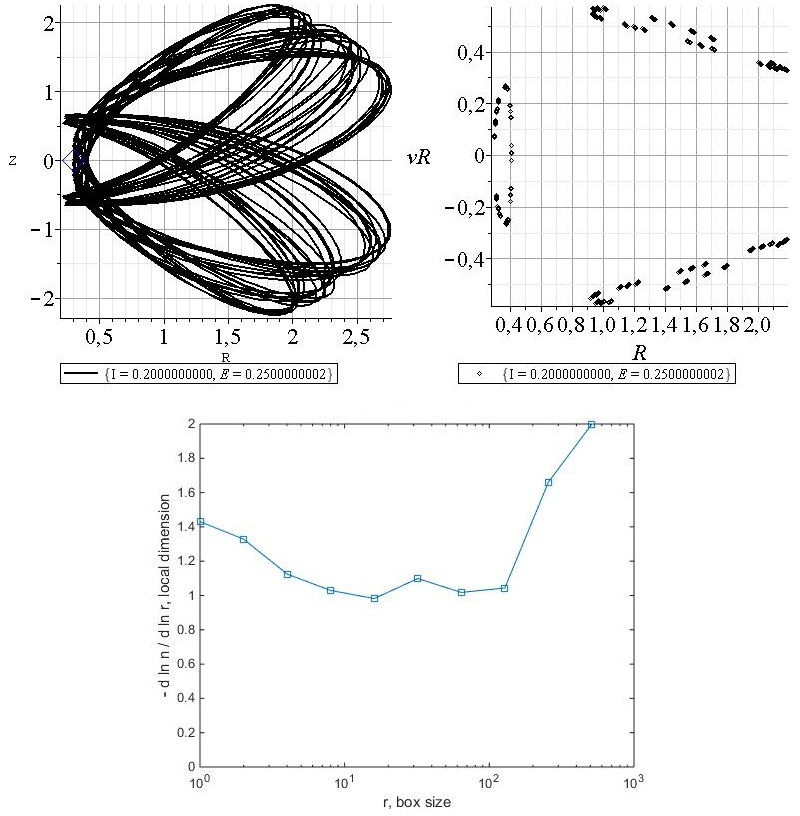
\includegraphics[width=\linewidth]{D:/diploma/tex/3/res/1_FULL.jpg}
\end{minipage}
\caption{Орита, сечение Пуанкаре и вывод box-count алгоритма. Фрактальная размерность $f = 1.8458 \pm 0.2889$}\label{stohast:1}
\end{figure}
}

{
\begin{figure}[H]
\centering
\begin{minipage}[t]{0.8\textwidth}
\centering
\includegraphics[width=\linewidth]{D:/diploma/tex/3/res/2_FULL.jpg}
\end{minipage}
\caption{Орита, сечение Пуанкаре и вывод box-count алгоритма. Фрактальная размерность $f = 1.9135 \pm 0.1538$}\label{stohast:2}
\end{figure}
}

{
\begin{figure}[H]
\centering
\begin{minipage}[t]{0.8\textwidth}
\centering
\includegraphics[width=\linewidth]{D:/diploma/tex/3/res/3_FULL.jpg}
\end{minipage}
\caption{Орита, сечение Пуанкаре и вывод box-count алгоритма. Фрактальная размерность $f = 1.8663 \pm 0.2603$}\label{stohast:3}
\end{figure}
}

На каждом из рисунков изображена орбита, соответствующее ей сечение Пуанкаре и вывод box-count алгоритма. По горизонтальной оси идет размер ячеек, а по вертикальной оси отношение натуральных логарифмов попавших в ячейку точек (count) к размеру ячейки (box). В подписях к рисунку указана фрактальная размерность $f$ для орбиты.\\

В третьей главе были главным образом построены сечения Пуанкаре для выбранного набора орбит и вычислена фрактальная размерность. Сечения Пуанкаре показали упорядоченный/нехаотический характер выбранных орбит. Однако фрактальная размерность оказалась дробной, что позволило сделать заключение об их нерегулярности.